\hypertarget{obsah-kurzu}{%
\chapter{Obsah kurzu}\label{obsah-kurzu}}

V~poslední kapitole si představíme vytvořený online kurz pro výuku datové analytiky. Tuto část dělíme do několika vzájemně provázaných částí, z~nichž každá reflektuje odlišnou oblast návrhu a~implementace online kurzu.

\hypertarget{prux16fchod}{%
\section{Průchod}\label{prux16fchod}}

V~první částí se zaměříme na obecný průchod kurzem -- popíšeme si, jak je kurz navržen po strukturální stránce a~jakým způsobem student prochází jednotlivými částmi.

Hlavní část kurzu je tvořena sedmi hlavními obsahovými bloky, z~nichž se každý zabývá jedním určitým tématem, které na sebe přímo navazují a~představují tak hrubou strukturu online kurzu (viz Obrázek \ref{digi-bloky}). Od studenta se tedy očekává lineární postup směrem od prvního do poslední obsahového bloku, nicméně je i~tak studujícímu umožněno procházet libovolný blok dle aktuálních potřeb (a~to ať už ty minulé např. z~důvodu ujasnění si již probraných témat nebo ty nenavštívené např. kvůli zjištění celkové časové náročnosti kurzu).

Mimo tyto ústřední bloky e-learning na začátku obsahuje úvodní text, jehož cílem je studenta navnadit ke studiu a~v~co největší stručnosti popsat obsah celého kurzu. Zároveň je pod touto úvodní kartou umístěn malý ukazatel progresu s~počtem splněných aktivit (viz další odstavec) spolu s~podkartou \emph{Užitečný tip}, která slouží v~rámci ekosystému kurzů Digiskills k~nasměrování na integrovaného chatbota (viz Obrázek \ref{digi-uvod}).

\begin{figure}[h]   
    \centering
    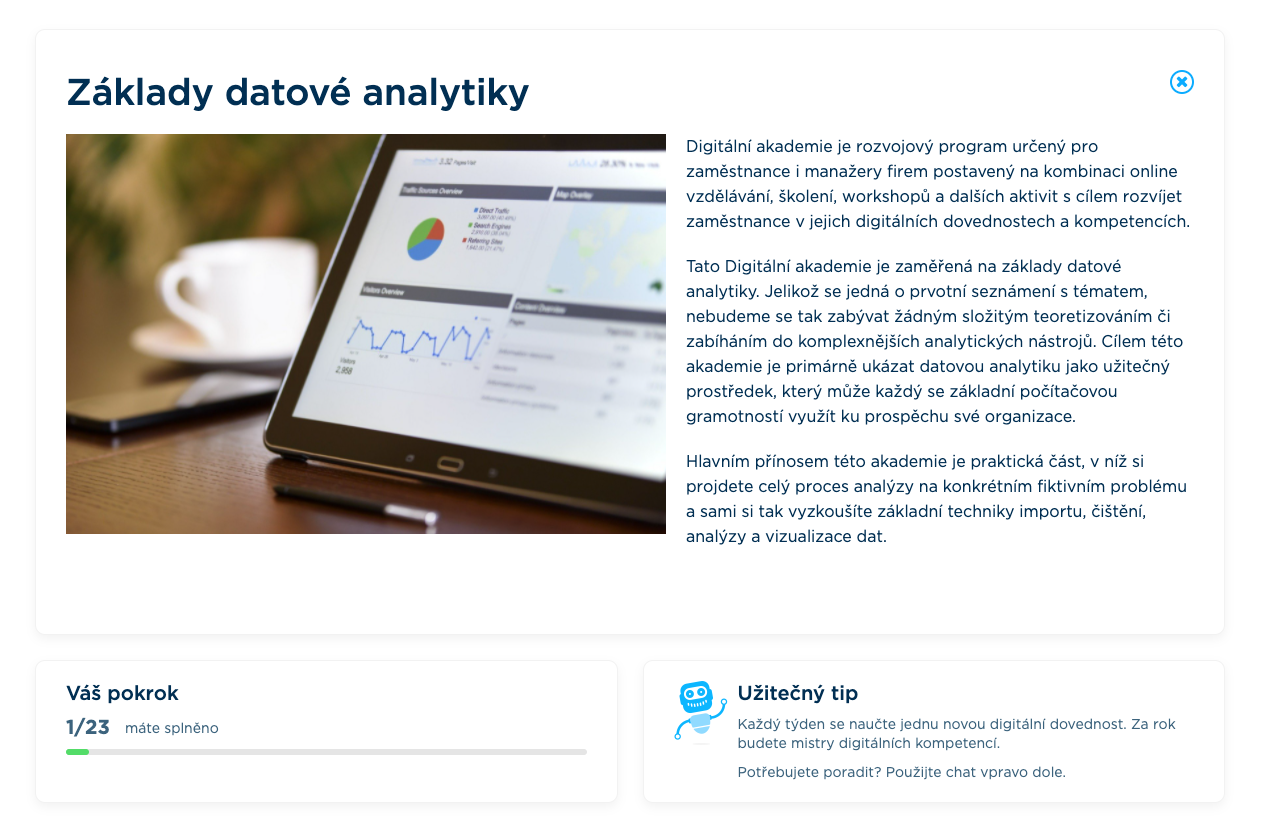
\includegraphics[width=\textwidth]{digi-uvod}  
    \caption{Úvodní obrazovka s~představením kurzu spolu s~ukazatelem progresu a~s~podkartou týkající se užitečného tipu}
    \label{digi-uvod}
\end{figure}

Základní jednotkou kurzu jsou pak již zmíněné aktivity, jež jsou vždy zanořeny do daného obsahového bloku (viz Obrázek \ref{digi-blok}). Těchto aktivit je v~celém kurzu v~současné chvíli 23 a~jsou do jednotlivých bloků logicky uspořádány dle následující šablony:

\begin{itemize}
\tightlist
\item
  úvodní aktivita, která představuje studentovi dané téma a~kontextualizuje jej v~rámci aktivit minulých a~následujících;
\item
  1--3 aktivity zpracovávající konkrétní část tématu;
\item
  1--2 závěrečné aktivity, jež shrnují dané téma a~pobízí studenta k~vlastní práci ať už prostřednictvím kvízů či praktických úkolů (viz Obrázek \ref{digi-aktivity}).
\end{itemize}

\begin{figure}[h]   
    \centering
    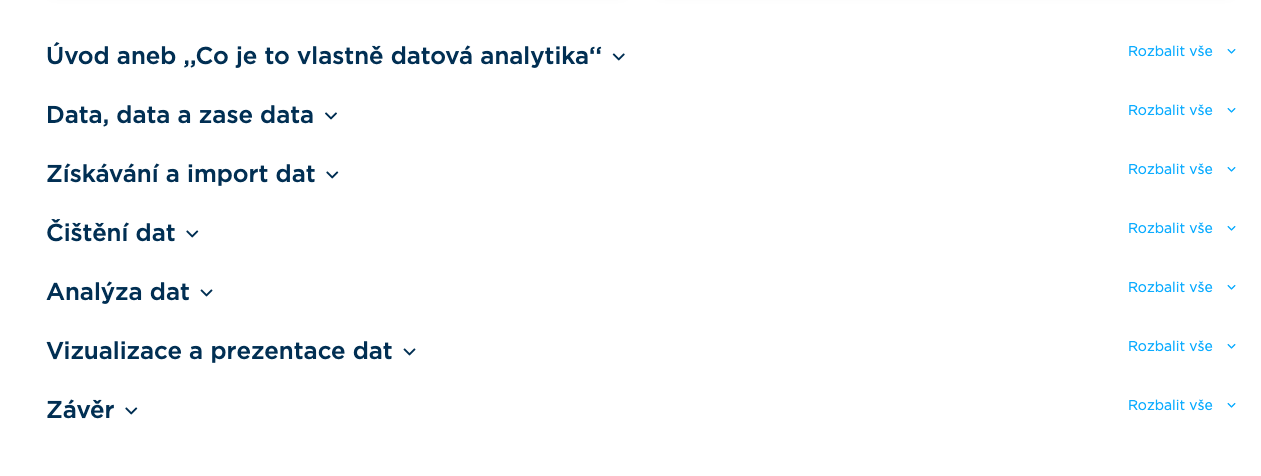
\includegraphics[width=\textwidth]{digi-bloky}  
    \caption{Nerozbalený výčet všech obsahových bloků}
    \label{digi-bloky}
\end{figure}

\begin{figure}[h]   
    \centering
    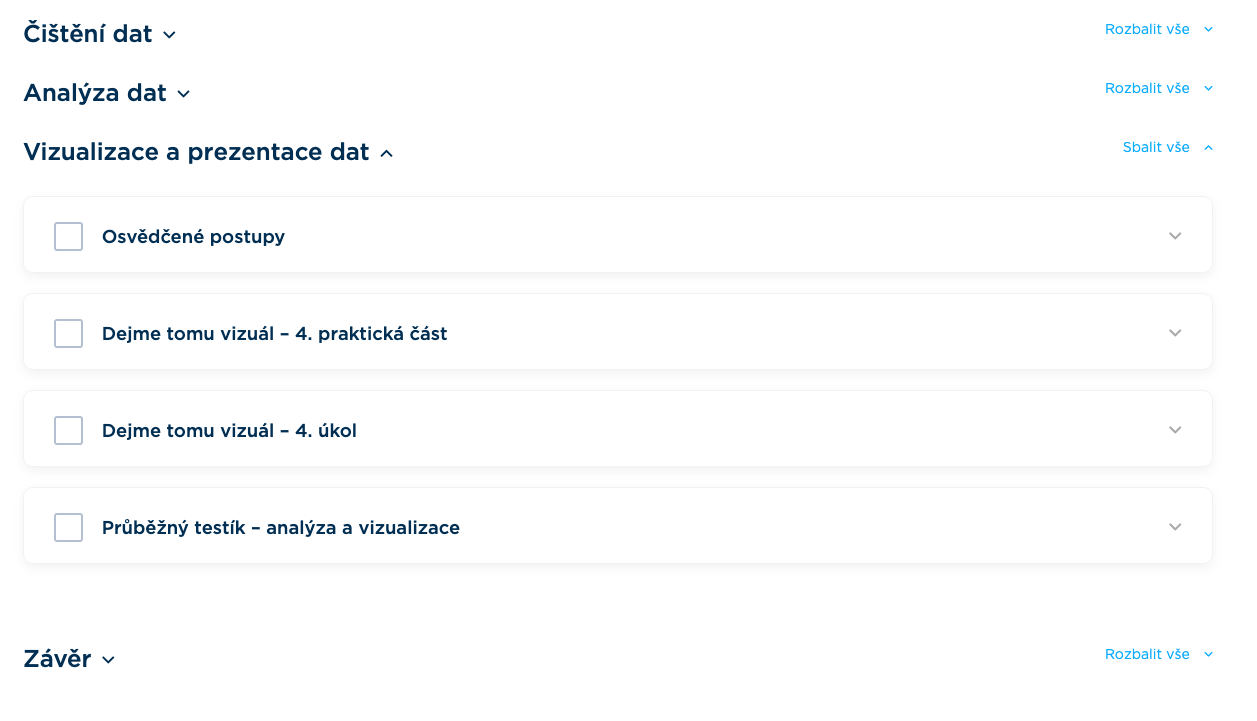
\includegraphics[width=\textwidth]{digi-blok}  
    \caption{Vnořené aktivity vztahující se ke obsahovému bloku Vizualizace a~prezentace dat}
    \label{digi-blok}
\end{figure}

\begin{figure}[h]   
    \centering
    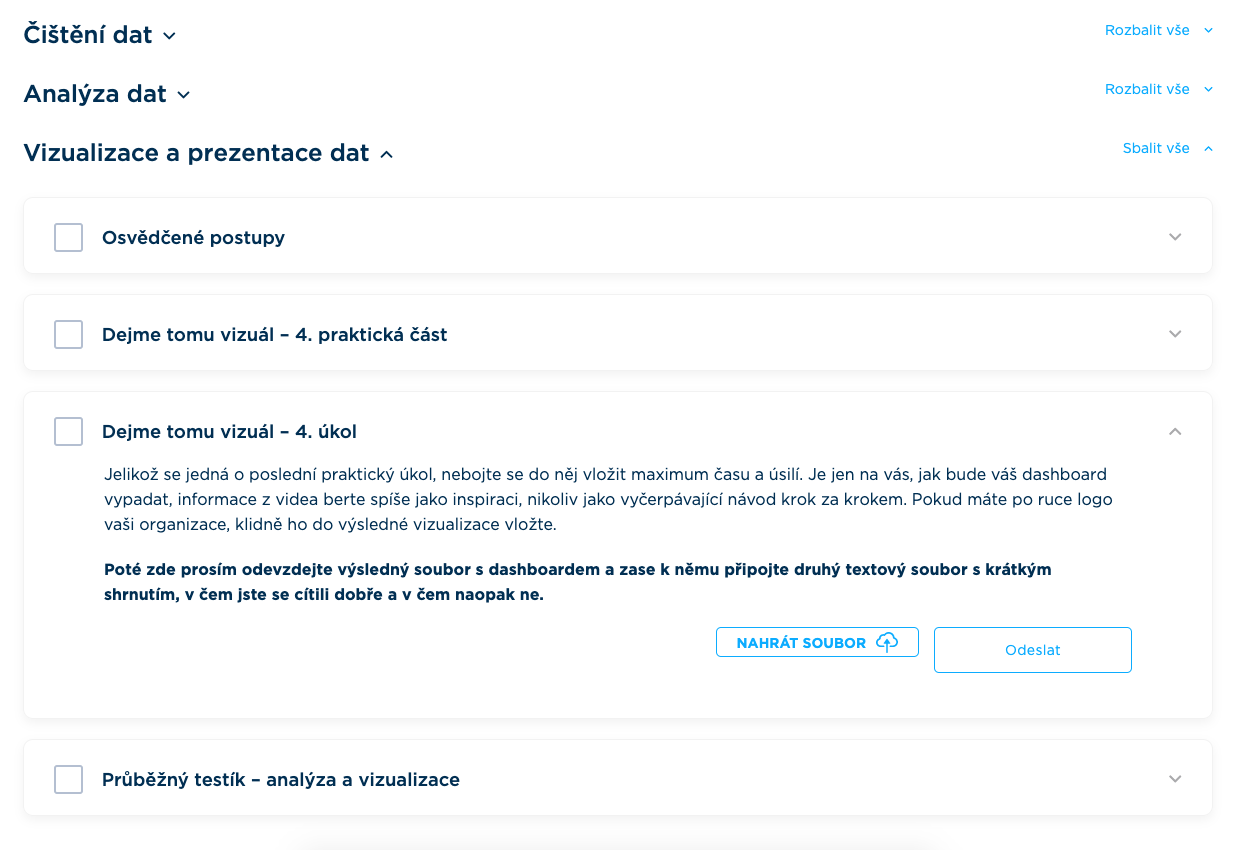
\includegraphics[width=\textwidth]{digi-aktivity}  
    \caption{Závěrečná aktivita, která obsahuje zadání praktického úkolu}
    \label{digi-aktivity}
\end{figure}

Všechny aktivity lze dále kategorizovat podle svého typu, který determinuje, jaká edukační komponenta je v~dané aktivitě využita. Kromě typů \emph{nahrát soubor} a~\emph{test typeform} (viz níže) musí student po dokončení vybrané aktivity vždy zatrhnout políčko \emph{Označit aktivitu za splněnou}, které aktualizuje progres studenta a~přesměruje ho na následující aktivitu.

V~našem online kurzu využíváme výhradně těchto pět typů aktivit, které jsme pro účely tohoto e-learningu vytvořili na základě výsledků z~provedené přehledové studie online kurzů:

\begin{itemize}
\tightlist
\item
  \emph{přečíst text} -- student musí pro splnění tohoto typu aktivity přečíst textový materiál, který je typicky doplněn o~vizualizace, jež téma obsahově doplňují, případně jej graficky člení pro větší přehlednost;
\item
  \emph{zhlédnout video} -- v~těchto aktivitách musí student zhlédnout video, které nejčastěji vysvětluje danou problematiku prostřednictvím praktických ukázek;
\item
  \emph{vložit text} -- tyto aktivity rozšiřují první typ, tedy textový materiál doplňují o~textové pole, do nějž musí student zadat odpověď na otázku vztahující se k~tématu;
\item
  \emph{nahrát soubor} -- aktivity tohoto typu jsou umístěny za výukovými videy, protože v~rámci nich student odevzdává vlastní vypracovanou práci spolu s~krátkou textovou reflexí\footnote{Krátkou reflexi jsme po odevzdání praktických úkolů začlenili z~toho důvodu, aby měl student možnost zapřemýšlet nad nově nabytými dovednostmi a~případnými nejasnostmi, které mohou spojeny buď s~probíranou problematikou anebo s~formátem samotného kurzu.};
\item
  \emph{test typeform} -- v~těchto aktivitách student vypracovává krátký kvíz, jehož cílem je připomenout hlavní znalosti a~dovednosti, které si v~rámci minulých aktivit osvojil. Při špatné odpovědi kvíz studenta naviguje ke konkrétní aktivitě, která látku vysvětluje, student může posléze svoji odpověď změnit a~znovu odpovídat (viz Obrazek \ref{digi-kviz} a~\ref{digi-kviz-0}).
\end{itemize}

\begin{figure}[h]   
    \centering
    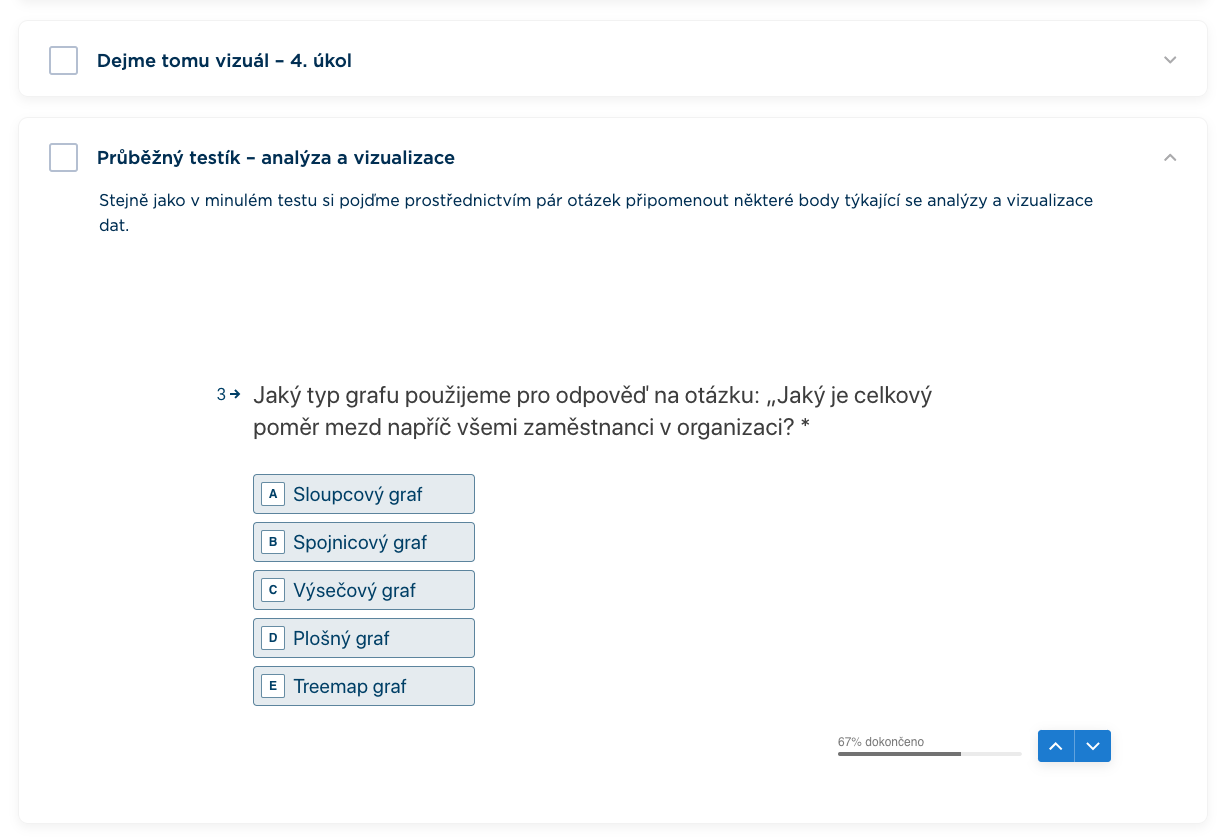
\includegraphics[width=\textwidth]{digi-kviz}  
    \caption{Příklad otázky z~průběžného kvízu týkající se tématu analýza a~vizualizace dat}
    \label{digi-kviz}
\end{figure}

\begin{figure}[h]   
    \centering
    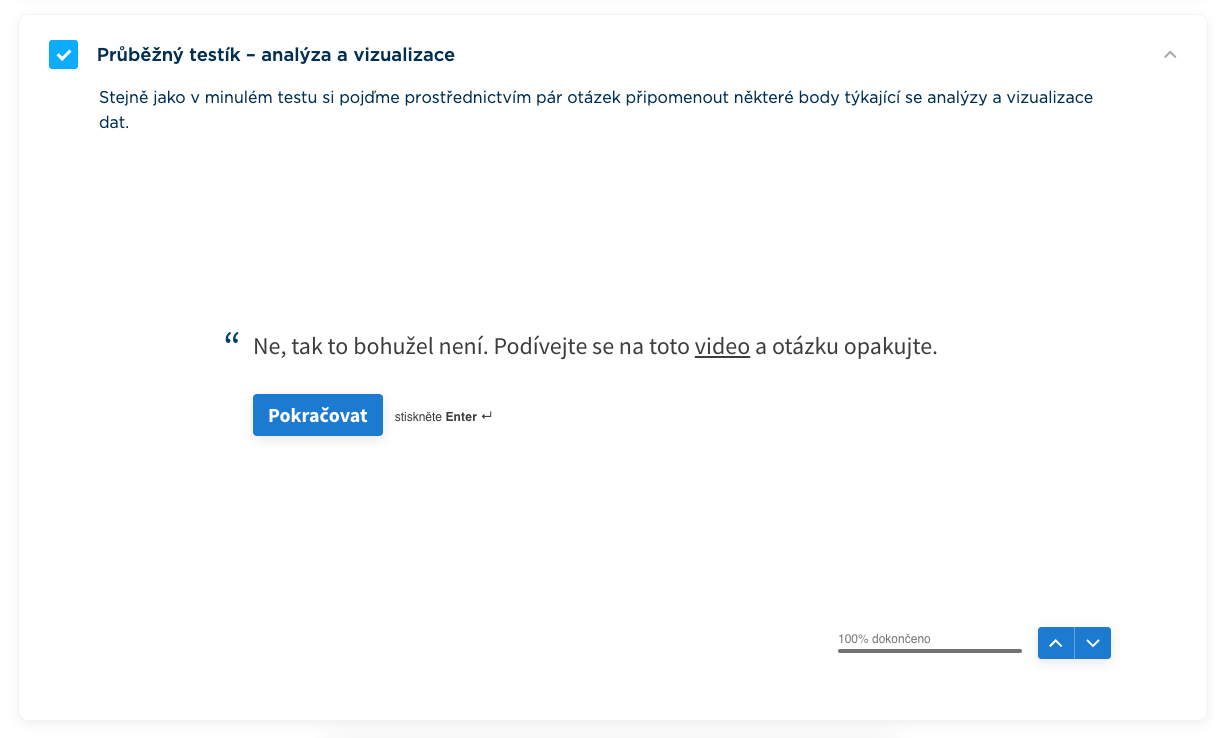
\includegraphics[width=\textwidth]{digi-kviz-0}  
    \caption{Příklad otázky z~průběžného kvízu týkající se tématu analýza a~vizualizace dat}
    \label{digi-kviz-0}
\end{figure}

Pro úspěšný průchod celým kurzem je zapotřebí mít splněné všechny dílčí aktivity včetně kvízů a~korektně odevzdané všechny praktické úkoly. Kurz byl navržen tak, aby byly všechny odevzdané úkoly zkontrolovány pověřenou osobou -- chceme tak docílit k~poskytnutí individuální zpětné vazby každému jednotlivému studentovi.

\hypertarget{moduly}{%
\section{Moduly}\label{moduly}}

V~této poslední podkapitole popíšeme jednotlivé obsahové bloky (dále jen moduly), které dělíme podle toho, jaký vzdělávací cíl splňují, a~tedy zda spadají do teoreticky nebo prakticky zaměřené části kurzu\footnote{Prostřednictvím celkové stylizace kurzu směřujeme k~co největší popularizaci tématu, proto jsou některé názvy jednotlivých obsahových bloků a~aktivit pojaty méně formálním způsobem.}.

\hypertarget{uxfavod-aneb-co-je-to-vlastnux11b-datovuxe1-analytika}{%
\subsection{Úvod aneb ‚‚Co je to vlastně datová analytika`\,`}\label{uxfavod-aneb-co-je-to-vlastnux11b-datovuxe1-analytika}}

První teoretický modul si klade za cíl uvést studenta do kontextu celého kurzu -- představuje mu možnosti online prostředí, vysvětluje, jak probíhá průchod kurzem, a~uvádí osnovu kurzu. Ještě před samotnou teorií týkající se úvodních témat datové analytiky je student seznámen se skutečností, že v~druhé, praktické části kurzu, bude sám participovat na svém vlastním řešení, prostřednictvím kterého by si měl osahat základní techniky datové analytiky.

V~dalších částech tohoto modulu je co srozumitelným způsobem vysvětleno, proč je důležité datovou analytiku v~organizacích využívat a~jakou přidanou hodnotu může mít při tvorbě firemních rozhodnutí. V~této části jsme se také zaměřili na koncept \emph{datově orientované organizace}, v~rámci kterého jsme se snažili vztáhnout téma datové gramotnosti právě na organizační prostředí a~znovu tak studenta motivovat ke studiu datové analytiky.

V~poslední aktivitě jsme se pak zmínili o~příbuzných pojmech, které se s~datovou analytikou pojí (např. \emph{Big Data} a~\emph{IoT}) a~jasně jsme vymezili příbuzené disciplíny jako jsou \emph{Data Science} a~\emph{Data Engineering}. Z~celkového hlediska tento modul naplňuje první dva vzdělávací cíle kurzu (viz cíle \ref{1-cil} a~\ref{2-cil}).

\hypertarget{data-data-a-zase-data}{%
\subsection{Data, data a~zase data}\label{data-data-a-zase-data}}

Druhý teoretický obsahový blok zpracovává problematiku spojenou s~definicí dat -- snaží se studentovi vysvětlit, co si pod pojmem data představit a~jakým způsobem lze data dělit a~kategorizovat podle daných potřeb. V~této sekci již studenta uvádíme do tématu prostřednictvím krátkého popularizačního videa a~následně pomocí stručného článku pobízíme k~zamyšlení, s~jakým typem dat student vlastně nejčastěji pracuje.

Na závěr modulu představujeme obsah praktické části kurzu, kterým je proces datové analytiky. Ve videu popisujeme jednotlivé fáze procesu a~snažíme se akcentovat fakt, že data nejsou totéž co informace, ale že ze surových dat informace získáváme právě prostřednictvím analýzy a~následné vizualizace. Tato část tak splňuje třetí vzdělávací cíl kurzu (viz cíle \ref{3-cil}).
